\documentclass{standalone}
\usepackage{../../../../preamble_formulas}

\begin{document}
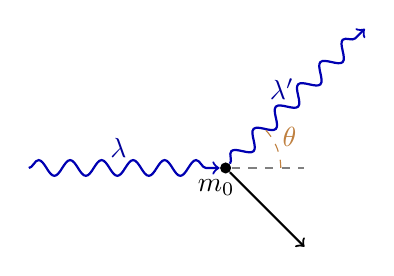
\begin{tikzpicture}
  % black circle
  \node[circle,fill=black,inner sep=0pt,minimum height=4pt](circ) at (0,0){};

  % photons
  \draw [->,blue!70!black,thick,decorate,decoration={snake,amplitude=1mm,segment length=4mm,post length=0.8mm}] (-2.5,0) --node[blue!60!black,anchor=south,pos=0.47]{$\lambda$}  (circ);
  \draw [->,blue!70!black,thick,decorate,decoration={snake,amplitude=1mm,segment length=4mm,post length=0.8mm}] (circ) --node[blue!60!black,anchor=east,pos=0.55]{$\lambda'$}  (1.7678,1.7678);

  % particle
  \draw[->, black, thick] (circ) --node[anchor=east,pos=0.2]{$m_0$} (1,-1);

  % horizontal line
  \draw[dashed, gray] (circ) -- (1,0);

  % angles
  \draw[domain=0:45,samples=50, brown,dashed] plot ({0.7*cos(\x)}, {0.7*sin(\x)});
  \node[brown,anchor=south west] at (0.6,0.15) {$\theta$};




\end{tikzpicture}
\end{document}
